\graphicspath{ {Background/Images/} }


\chapter{Background}
\label{cha:background}

\section{Introduction}
In this chapter we introduce important concepts which are needed to understand our approach. These concept can be used to solve problems described in chapter \ref{cha:context}. \\

We start with explaining some background knowledge as time series and machine learning. We then focus on neural networks, which is a machine learning approach. The main part to understand our approach is the introduction of Word2vec. This is then used to introduce Deepwalk as an extension on Word2Vec.


\section{Background Knowledge}

	\subsection{Time Series Analysis}
A time series consists of data points over a certain time period. We refer to this as a sequence of states. Where a state represents a data point and can differ from a single value to more complex representations like pictures. \\
The domain of time series analysis handles around extracting information or relations from a time series. It can have different goals like forecasting, classification, or exploratory. \\

A medical history of a patient can be seen as a time series. This means that methods applied on time series are also applicable on the medical data to find patterns.

	\subsection{Machine Learning}
Machine learning is a data driven approach with as goal to build a model which can be	used to make predictions or decisions. Note that this model can be used to predict outcomes of time series. This task is done by algorithms which are able to learn models based on examples given by the designer. Based on the examples, machine learning aims to tackle $3$ types of problems, namely supervised learning, unsupervised learning, and reinforcement learning. \\
Supervised learning is concerned with the learning task where there are examples given with their corresponding label. Unsupervised learning is similar to supervised learning only no labels are given. We won't go into reinforcement learning. \\
We can also classify the problems according to the desired output of our model. Those main tasks consist of classification, regression, and clustering. \\
	
We mention some used methods in the field of machine learning. These are used in all above mentioned problems. \\
In the field of classification neural networks are used to achieve state of the art results. For regression, Support Vector Machines can be used. One of the most popular methods for clustering is K-means. 
	
	
	\subsection{Neural Networks}
	
A neural network is a machine learning approach based on biological neural networks. 


		\subsubsection{Perceptron}

The basic component of a neural network is a perceptron. A perceptron takes multiple binary inputs and has a single binary output (see figure \ref{fig:perceptron}). Each input has a corresponding real numbered weight. The output is decided on the following equation:

\begin{equation} 
output =
  \begin{cases}
    0       	& \quad \text{if } \sum_j w_jx_j \leq \text{ threshold}\\
    1  		& \quad \text{if } \text{if } \sum_j w_jx_j > \text{ threshold}\\
  \end{cases}
\end{equation}
	
\begin{figure}[H]
	\centering
	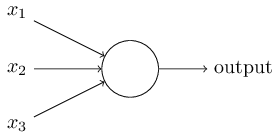
\includegraphics[width=0.4\textwidth]{perceptron.png}
	\caption{Simple presentation of a perceptron \cite{NNintro:online}}
	\label{fig:perceptron}
\end{figure}

We can build a network by connecting multiple perceptrons (see figure \ref{fig:multiplePerceptrons}). By building these networks, more complex decisions can be made. The reason for this, is that once there are atleast $3$ layers of perceptrons, the network can find non-linear relations between the input and output.

\begin{figure}[H]
	\centering
	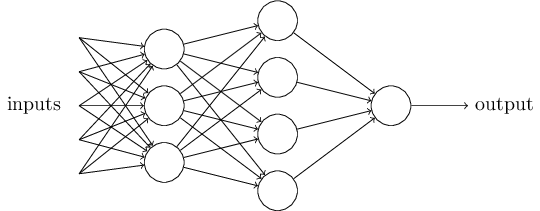
\includegraphics[width=0.8\textwidth]{multiplePerceptrons.png}
	\caption{More complex network made by connecting multiple perceptrons \cite{NNintro:online}}
	\label{fig:multiplePerceptrons}
\end{figure}

Now we have seen how a general network is constructed, we look at some vocabulary. \\
In figure \ref{fig:networkArch}, we see a four-layer network. As mentioned on the figure, we call the first layer the input layer, the last layer the output layer, and the layers in between are called hidden layers. Sometime multiple layer networks are referred to as multilayer perceptrons or MLPs.

\begin{figure}[H]
	\centering
	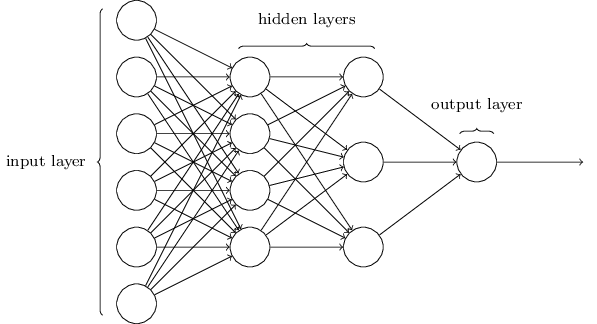
\includegraphics[width=0.8\textwidth]{networkArchitecture.png}
	\caption{General vocabulary for a multilayer network \cite{NNintro:online}}
	\label{fig:networkArch}
\end{figure} 		


		\subsubsection{Training a network}
		
To train a neural network, we input an example with a known label. The network will calculate a certain output based on the current weights. When this output is incorrect, it should be possible to adjust the weights with as effect that the network now has as output the correct label. Note that the change in weights, should only effect the output by a small bit (see figure \ref{fig:smallChange}). The reason for this is that otherwise all the previous images could now be labeled incorrectly. So, the concept of training a neural network means, adjusting the weights in a way that the behavior of the network doesn't change completely on the previous seen pictures but that the current picture is labeled correctly.

\begin{figure}[H]
	\centering
	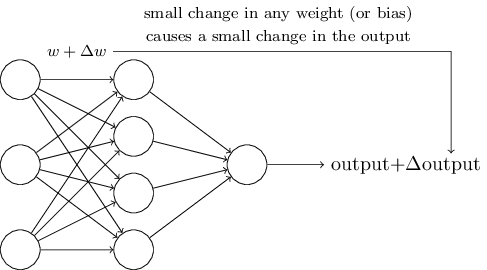
\includegraphics[width=0.8\textwidth]{smallChange.png}
	\caption{Small change on the weights, only has a small impact on the output \cite{NNintro:online}}
	\label{fig:smallChange}
\end{figure} 

To achieve this effect, we change our known perceptrons to sigmoid neurons. A sigmoid neuron has the same basics as a perceptron. It still has inputs but now it also has a bias $b$. The inputs still have weights but the weights can now range between $0$ and $1$. The output is now calculate with $\sigma(w*x+b)$ where $\sigma$ is the sigmoid function. This results in the following formula: 

\begin{equation} 
\frac{1}{1+exp(-\sum_j w_jx_j-b)}
\end{equation}

The sigmoid function makes it possible to calculate the gradient and makes the output a linear combination of $\Delta w_j$ and $\Delta b$ as $\Delta output$ is approximated by 

\begin{equation} 
\Delta output \approx \sum_j \frac{\partial output}{\partial w_j}\Delta w_j + \frac{\partial output}{\partial b}\Delta b
\end{equation}

Because of the linearity, it is now possible to choose changes for the weights and biases to achieve a correct output. By adjusting the weights, we will train our network to achieve a higher accuracy.
		
	\subsection{Backpropagation}
	
Backpropagation is an algorithm which is used to train neural networks. It calculates the gradient of a chosen cost function with respect to the individual weights. With the gradient, the weights are updated and the cost function is minimized.

		\subsubsection{Terminology}
		
We use $w^l_{jk}$ to denote the weight corresponding to the connection between the $k^{th}$ node in the $(l-1)^{th}$ layer to the $j^{th}$ node in the $l^{th}$ layer. We use $b^l_j$ for the bias of the $j^{th}$ node in the $l^{th}$ layer and $a^l_j$ for the activation of the $j^{th}$ node in the $l^{th}$ layer. See figure \ref{fig:termNN}.

\begin{figure}[H]
	\centering
	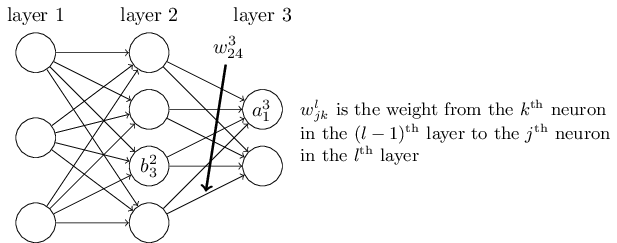
\includegraphics[width=0.8\textwidth]{termNN.png}
	\caption{Visual representation of the terminology for a neural network \cite{NNintro:online}}
	\label{fig:termNN}
\end{figure} 

We can now convert these notation to a vector representation. We remove the indexes for the node numbers which results in the following:

\begin{equation} 
a^l = \sigma (w^la^{l-1}+b^l)
\end{equation}

		\subsubsection{Cost function}
		
As mentioned before, backpropagation has as goal to calculate the partial derivatives of the cost function $C$ with respect to each weight and bias. \\
The cost function has to fulfill certain criteria. The first one is that it needs to be possible to write it as a summation over cost functions for individual training examples. Secondly, it needs to be derivable. And lastly, the cost function is a function of the activations of the last layer. 


		\subsubsection{Fundamental equations}

Backpropagation has 4 equations. They allow us to calculate the error for each node and adjust the weights based on the gradient descent. \\

First we calculate the error of each node which is based on how much the cost function is influenced by each activation and on how much the activation function is influenced by $z_j^L$:

\begin{equation} 
\delta^L_j = \frac{\partial C}{\partial a^L_j} \sigma'(z_j^L)
\text{ with }
z_j^L = \sum_k w^L_{jk}a^{L-1}_k+b^L_j
\end{equation}

This can be written as a neat vector equation:

\begin{equation} 
\delta^L = (a^L-y) \circ \sigma'(z_j^L)
\end{equation}

The next equation explains why the algorithm is called backpropagation. The equation calculates each layers error vector based on the layer after it, it propagates the error back over the layers:

\begin{equation} 
\delta^l = ((w^{l+1})^T\delta^{l+1}) \circ \sigma'(z_j^L)
\end{equation}

With those 2 equations we calculate the error in each layer of the neural network. Those errors can be used to calculate the derivatives of the cost function with respect to the weights and the biases:

\begin{equation} 
\frac{\partial C}{\partial w^l_{jk}} = a^{l-1}_k \delta^l_j.
\end{equation}

\begin{equation} 
\frac{\partial C}{\partial b^l_j} = \delta^l_j.
\end{equation}

When the derivatives are calculated, we can apply the gradient descent and update the weights and biases accordingly. This process represents the learning of a neural network.


\section{Word2Vec}
\label{sec:word2vec}

\subsection{Motivation}

In natural language processing tasks, a good representation of words helps learning algorithms perform better. A representation is learned which maps words to vectors in a low-dimensional space compared to the vocabulary size. In this representation, we try to map context-similar words close to each other in the new vector space. \\
We could say in an informal way: a linguistic background is made which the learning algorithm can use.


\subsection{Skip-gram}

There are two main models used for word2vec \cite{w2vOriginal:article}, namely Continuous Bag-of-Words (CBOW) and the Skip-Gram model. \\
The first one tries to predict a word if a context is given (ex. predict Paris when capital France is given). And the second one does the inverse of this approach \cite{w2vModels:article}. Empirical results have shown that the Skip-Gram model tends to do better on larger datasets \cite{w2vReason1:online} and gives a better representation for infrequent words \cite{w2vArchive:online}. In medical data there are often infrequent cases which are important. For those reasons, we choose to go further with the Skip-Gram model. \\

So one way of learning a word2vec representation of a corpus $Text$, is by using the skip-gram model. \\
Based on given words $w$ and their contexts $c$, we set the parameter $\theta$ of $p(c|w;\theta)$ to maximize:

\begin{equation} 
\arg \max_{\theta} \prod_{(w,c \in D} p(c|w;\theta)
\end{equation}

with $D$ the set of all word and context pairs we extract from the corpus.\\
Here we also note that $p(c|w)$ is indeed the chance of a context appearing after seeing a specific word as mentioned before.

\subsubsection{Finding word-context pairs}

Given a sequence of words, we define their context based on n-gram \cite{w2vNgram:article}. In figure \ref{fig:ngram}, n-gram is explained on the sentence "This is a sentence". 

\begin{figure}[H]
	\centering
	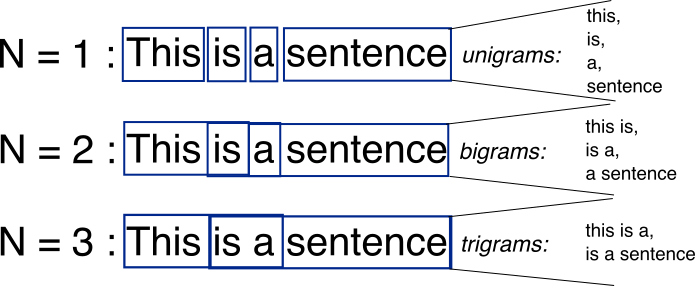
\includegraphics[width=0.8\textwidth]{ngram.png}
	\caption{Explanation of n-gram \cite{w2vNgram:online}}
	\label{fig:ngram}
\end{figure} 

For the Skip-gram model, we define the context of a word $w_t$ as $w_{t+j}$ with $j$ between $-c$ and $c$. A larger $c$ results in more training examples and thus can lead to a higher accuracy but will have a longer training time.


\subsubsection{Parameterization}

We start with rewriting the conditional probability using soft-max:

\begin{equation} 
p(c|w;\theta) = \frac{e^{v_x*v_w}}{\sum_{c' \in C}e^{v_{c'}*v_w}}
\end{equation}

where $v_c$ and $v_w$ are vector representations for $c$ and $w$, and $C$ is the set of all available contexts. This means that the parameters $\theta$ are $v_{c_i}$ and $v_{w_i}$. Computing the optimal parameters is very expensive because you need to calculate this over all contexts $c'$. We also switch from product to sum by taking the logs:

\begin{equation} 
\arg \max_{\theta} \sum_{(w,c) \in D} \log p(c|w;\theta) = \sum_{(w,c) \in D} (\log e^{v_c * v_w} - \log \sum_{c'} e^{v_{c'}*v_w})
\end{equation}

\subsection{Negative Sampling}

To compute the vectors using the Skip-gram model more efficiently, we introduce negative sampling \cite{w2vExplained:article}. \\
Instead of calculating $\sum_{c' \in C}e^{v_{c'}*v_w}$ over all contexts, we make a set $D'$ which consists of randomly sampled word-context pairs. With this new set, we remove the costly term $\sum_{c' \in C}e^{v_{c'}*v_w}$ and replace it with $\sum_{(w,c) \in D'}e^{v_{c'}*v_w}$. \\

In a less formal way: we are not making sure that if words appear in the same context, their vectors are more similar than all the other word vectors, but only of several vectors chosen randomly. This makes the Skip-gram model usable in terms of speed.


\subsection{Neural Networks}

When the word2vec algorithm is trained using the Skip-gram model, one will have a lookup table. This table contains the mapping of words to their vector representation. This lookup table can be found by training a 2-layer neural network with as goal function the function described in the previous section. The training can be done with Gradient Descent for example. \\
The trained 2-layer neural network can be placed in front of another neural network \cite{w2vNN:online}. It will convert the words to their vector representation and feed into the next neural network. It is empirically shown that this can improve the results of the neural network by putting the lookup table in front of it. As mentioned before, in a way, you offer background knowledge to the neural network.

\newpage
\section{DeepWalk}

DeepWalk is an approach where graph structured data is transformed into sequences of vertices \cite{deepwalkMain:article}. Word2vec is then applied on those sequences to learn a good vector representation for the vertices. \\

In figure \ref{fig:dwAlgo}, we see an overview of the DeepWalk algorithm. It exist of two parts. 

\begin{figure}[H]
	\centering
	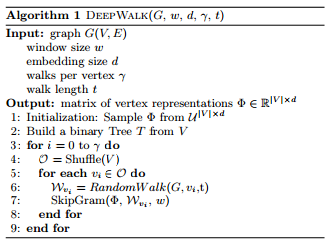
\includegraphics[width=0.7\textwidth]{dwAlgo.png}
	\caption{Overview of the DeepWalk algorithm \cite{deepwalkMain:article}}
	\label{fig:dwAlgo}
\end{figure} 

First a random walk generator. For each vertex $v_i$ of the graph $G$, it will generate a random walk of length $t$. It will do this $\gamma$ times but the order to which the vertices are traversed, is randomly ordered each pass. With those walks, a sequence of vertices is generated. \\
Secondly, those vertices are used for word2vec. This process is explained in section \ref{sec:word2vec}.


\section{Conclusion}
In this chapter we talked about general machine learning concepts and focused on Word2Vec. We conclude that Word2Vec is used to find good representation of words based on their context. It also causes that similar words will be close to each other in this new representation. \\

With the concepts explained in this chapter, we can introduce our approach in the next chapter. This approach is used to find patterns in EHR data.



%%% Local Variables: 
%%% mode: latex
%%% TeX-master: "thesis"
%%% End: 
